\chapter{Alignment}
\label{chapter:hps:alignment}

Particle detectors used to ``track'' particles (often called ``trackers'') largely operate by
precisely measuring the position of the particle at several different points along its trajectory.
From these position measurements, we are able to extract other, more physically helpful,
measurements such as momentum and charge (as long as the particles move through a magnetic field so
their resulting trajectory is curved in a well known shape). We will not go into the process of
converting these position measurements into trajectories of individual particles (``tracks'') or
estimating physical variables of these tracks. Instead, this serves as motivation: without precise
knowledge of position, we are unable to precisely estimate momenta of particles -- significantly
impacting the capabilities of the experiment.

We need all of these position measurements to be relative to the same reference point (i.e. in the
same coordinate system); thus, the process of measuring particle positions is practically done by
combining two position measurements.
\begin{enumerate}
  \item Position relative to individual pieces of the tracker (here called ``sensors'')
  \item ``Global'' position of these sensors
\end{enumerate}
More specifically, the software we use to deduce physical measurements from the data
output by a tracker consists of a detector model (which stores the positions of all
sensors in the same coordinate system) and a series of algorithms we can apply to
this detector model along with data from the sensors.

While there are different stragies to measure position within an individual sensor of the tracker
(e.g. pixel vs strip tracking detectors), this measurement is not the limiting factor in the
context of this chapter and is often the measurement whose precision is easier to characterize
since the individual sensors can be designed, built, and tested individually for a pre-determined
precision.

The second position measurement -- the global position of the sensors themselves -- is where a lot
of complexity arises. We construct the detector and thus know where we put the sensors, but placing
them into position with the precision we desire is extremely difficult (not to mention their
position could shift slightly once the magnet is turned on).

We can gain some understanding of the position precision required with the help of
\cref{fig:momentum-error-from-position-error}. There, we see that the momentum error roughly scales
by a factor of five relative to the position error and, as the position error goes up, the
momentum's distribution starts to distort away from a normal shape. In addition to the scaling of
the \emph{relative} error, the overall scale of these measurements are an important factor as well.

\begin{figure}
  \centering
  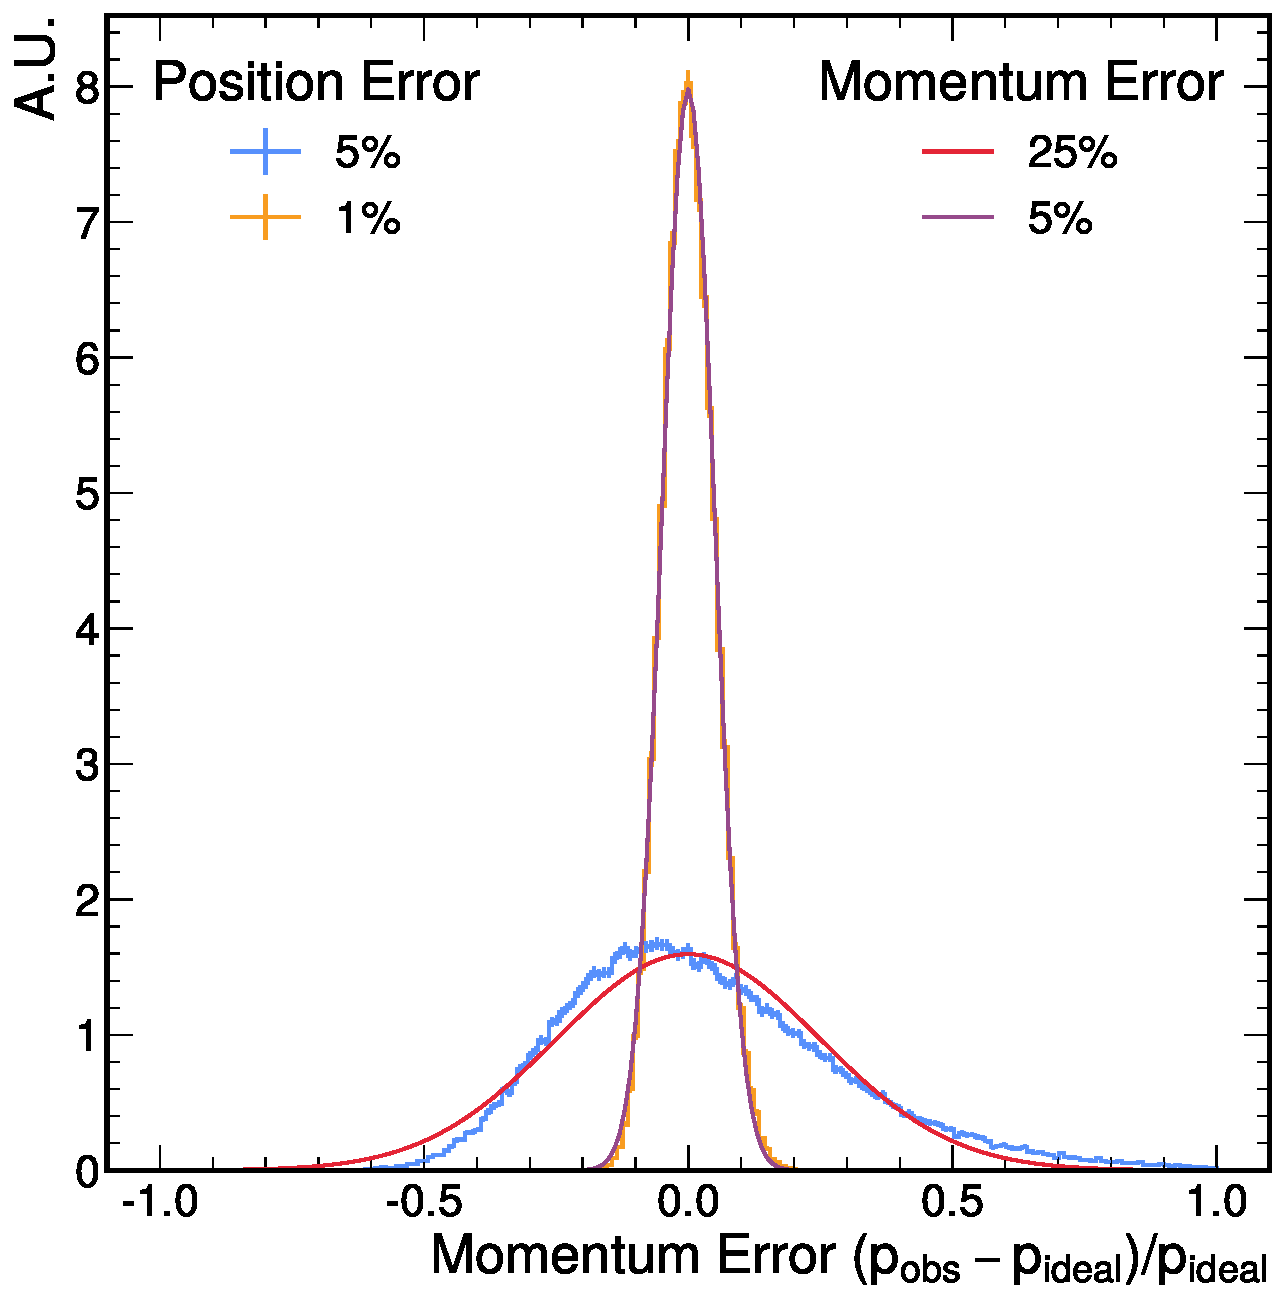
\includegraphics[width=0.5\textwidth]{one-offs/position-momentum-uncertainty/momentum-error-from-position-error.pdf}
  \caption{
    Momentum error derived from injecting a certain amount of position error
    (blue and orange) compared to normal distributions (red and purple)
    with known momentum error.
    These distributions are normalized to have unit integrals.
    The trials were done in a simplified experimental model with quantities
    similar to \ac{hps}: a \qty{2}{\giga\electronvolt} electron curving within a
    \qty{1}{\tesla} magnetic field, the sensors measuring the position were
    separated by \qty{5}{\centi\meter} but their separation were also allowed to
    deviate from the true value by the position error given.
  }
  \label{fig:momentum-error-from-position-error}
\end{figure}

Just to achieve a rough estimate of the scale of these position measurements, consider a
\qty{2}{\giga\electronvolt} electron curving within a \qty{1}{\tesla} magnetic field. This electron
would then have a \qty{6.6}{\meter} radius of curvature due to this magnetic field, meaning the
position measurements within sensors separated by \qty{5}{\centi\meter} would change relative to
one another by \emph{less than} \qty{1}{\milli\meter}. This absolute measurement of
$\sim\qty{100}{\micro\meter}$ combined with the necessary \qty{1}{\percent} relative error means we
need to know the position measurements to the level of \qty{1}{\micro\meter}.

While we can determine the position of these sensors within millimeter precision during
construction, gaining another few orders of magnitude in precision knowledge of position is not
feasible with physical-access tools. \todo[phrasing]{not sure how to separate design position from
  construction survey from post-construction survey from in-situ alignment measurements with beam
  particles.} This motivates another measurement ``tool'' that allows us to determine (or more
accurately, constrain) the position measurements of our sensors.

\section{Alignment Procedure}
The tool that we choose to use is the same particles that we will use the tracker to study for our
experimental goals. The one change is instead of using the tracker to measure the properties of
these particles, we will select particles according to our knowledge of their properties so that we
can use them to constrain the position of the tracker sensors.

This constraint is born out of concrete connection between the physical kinematics of the particles
and the positions they record in the tracker sensors. We can imbue our knowledge of the shape of
particle trajectories in magnetic field into the mathematical form of the equations that are fit to
the position measurements. If the sensors in the detector model were in slightly different
positions that where they are in the real detector, the data would present fits that are not as
good (quantitatively, have a higher $\chi^2$). With this in mind, we can slightly ``move'' the
sensors in the detector model with focus once improving the fits in the data (lowering the
$\chi^2$). In order to account for the fact that individual tracks may still vary due to our
imperfect knowledge of their trajectory shapes (e.g. the trajectory shape assumes only soft
interactions with the detector material but some tracks could have harder interactions distorting
their trajectory), we do this procedure over many tracks at once and focus on improving all of
their fits (minimizing the sum of their $\chi^2$).

This technique relies on the movements of the sensors to be small. The process can easily fall into
a so-called ``Weak Mode'' where our quantitative measure of how good the fits are is achieving a
locally minimum value, but the trajectories do not actually align with data. This motivates a
multi-stage approach to alignment after a tracking detector has already been built.

\begin{enumerate}
  \item \textbf{Survey}: Directly measure positions of the sensors relative to other
        detector components as precisely as possible.
  \item \textbf{In-Situ Alignment}: While only allowing for certain types of movements,
        minimize the total $\chi^2$ of well-known tracks.
\end{enumerate}

Since physical measurements obtaining the precision we require are so difficult, the survey is
often split into multiple, cascading measurements as well For example, the positions of the sensors
are precisely determined relative to their mounting brackets which are then measured relative to
the holding frame which is then measured relative to the global coordinates within which the
experiment operates.

The second stage where we perform small movements of the sensors in order to optimize the fit of
our data to our software detector model is also broken into many smaller stages. The most common
way is to only allow a certain set of physically motivated movements to occur during certain
alignment iterations. This can allow us to ``walk'' towards a detector model that is more aligned
with the physical detector while maintaining physical understanding of the changes being made.

\section{Detector Visualization}

In some sense, both of these stages inform the detector model and, as such, a critical piece of
alignment is a quantitative visualization of this detector model and how it is being modified.
\cref{fig:example-det-vis-abs} demonstrates a quantitative visualization used within \ac{hps} where
the positions and orientations of all the sensors within a specific coordinate system are shown.
This visualization is helpful for verifying that the detector model being used within the software
is placing the sensors in expected positions and orientations. For example, we observe the $y$ and
$z$ positions steadily increasing as the layer number of the sensor increases -- representing the
opening angle as designed within \ac{hps}. Additionally, we see many of the sensors ``flipped''
along one or more directions (the angle is $\pi \approx \qty{3141}{\milli\radian}$) which can be
double checked against design and construction.

\begin{figure}
  \centering
  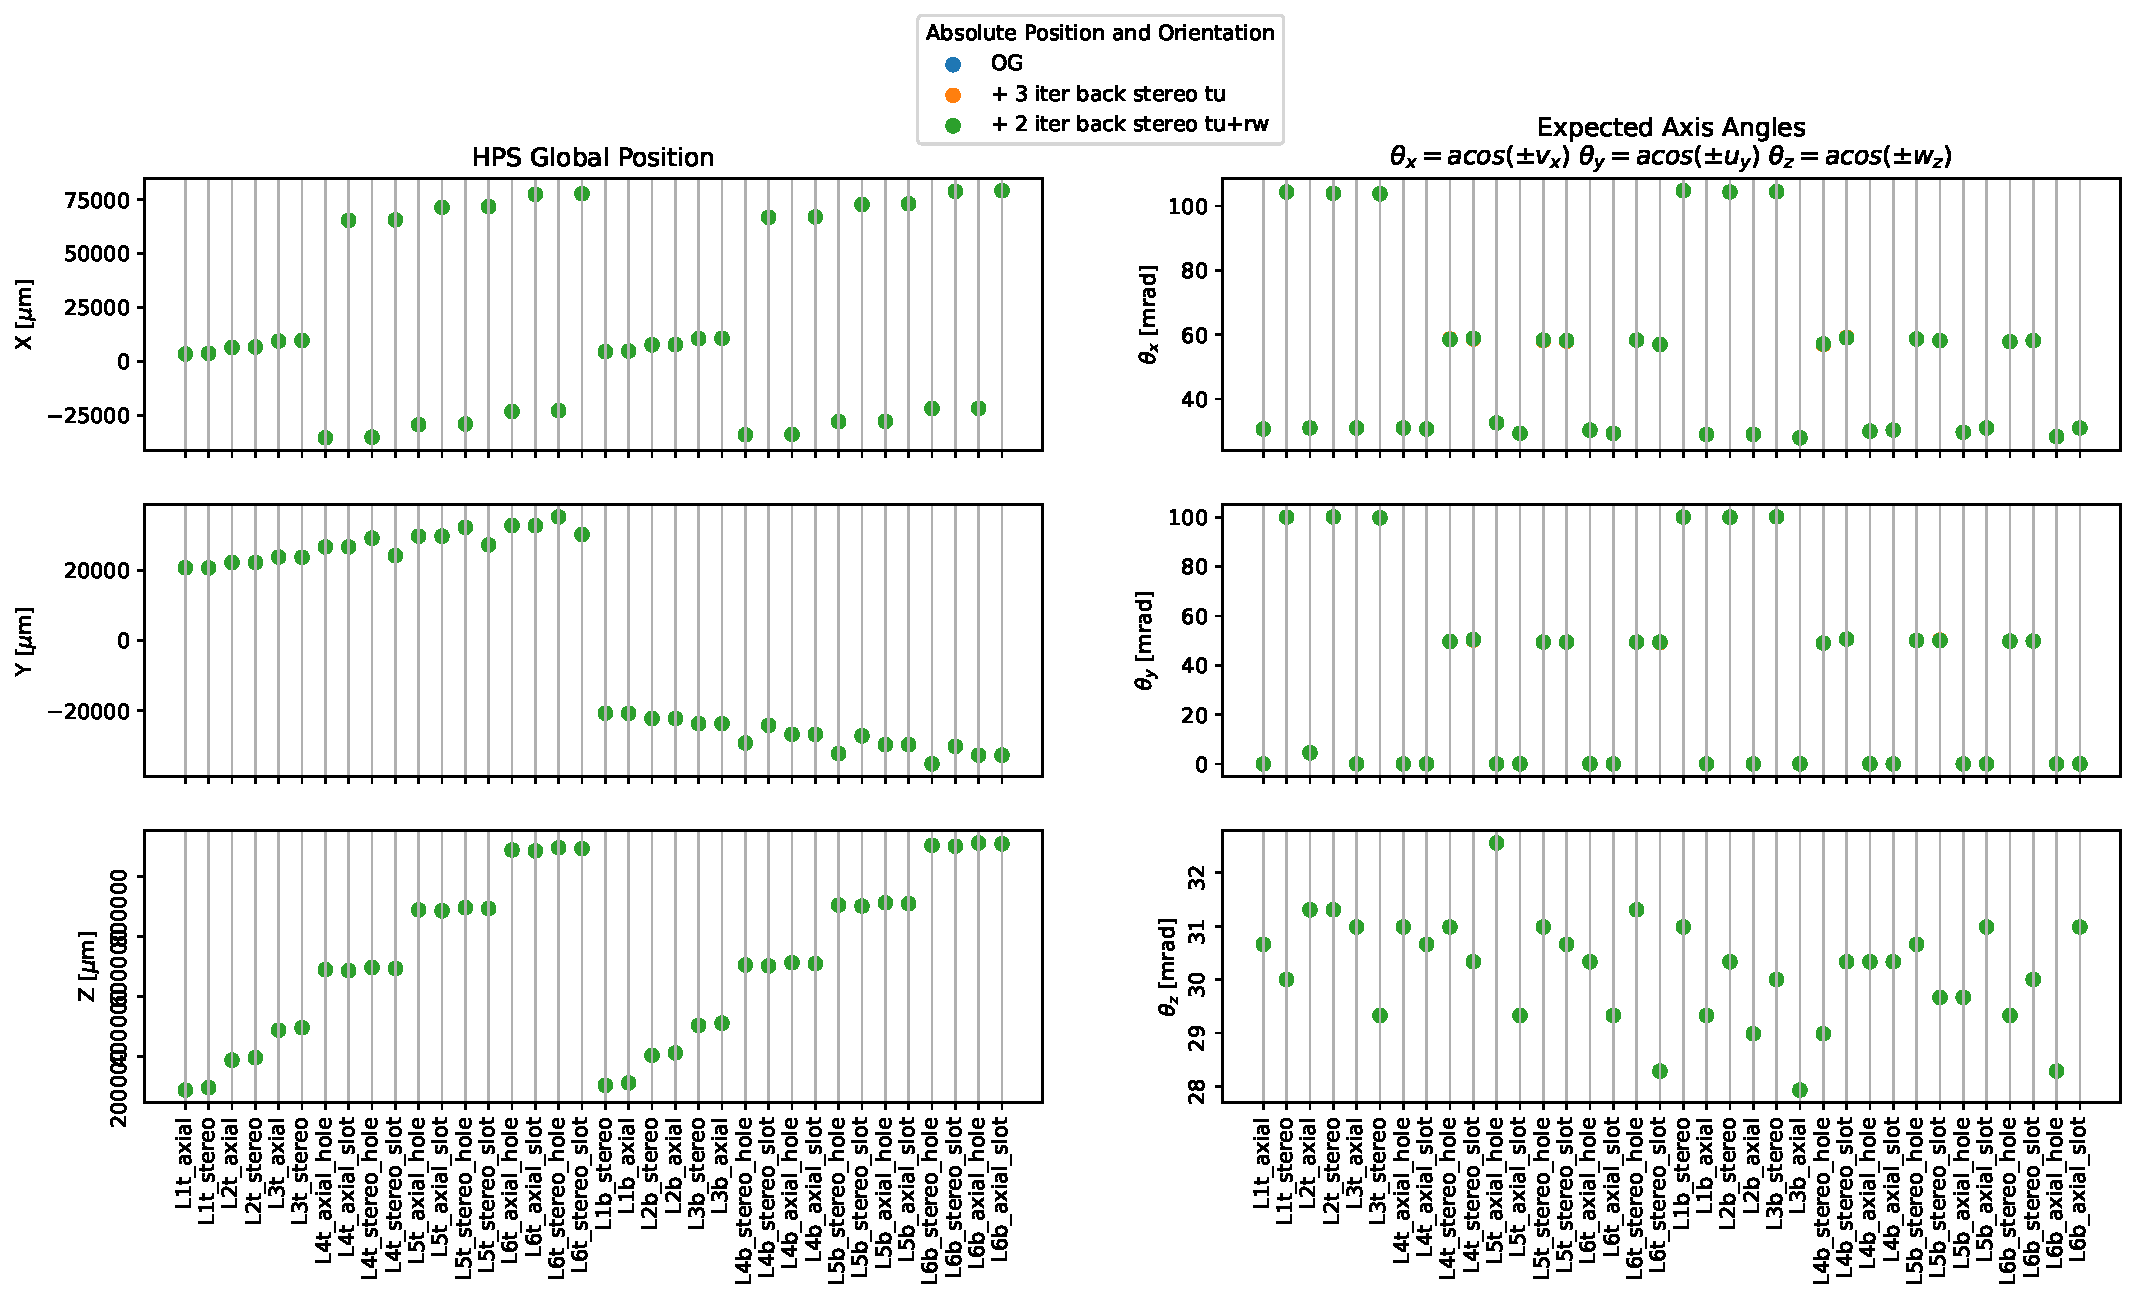
\includegraphics[width=\textwidth]{figures/hps/alignment/example-det-vis-abs.pdf}
  \caption{Plotting all six global coordinates completely specifying position and orientation
    of each of the sensors in the \ac{hps} tracking detector. Three different versions of the
    in-software detector model are plotted; however, on this scale, they all overlap one another.}
  \label{fig:example-det-vis-abs}
\end{figure}

Of more specific help is looking at the differences of these coordinates between multiple versions
of the detector model. \cref{fig:example-det-vis-diff} demonstrates this strategy by subtracting
the coordinates of the original detector model (``OG'') from the subsequent attempts to further
align it. Specifically, we can observe that the alignment iterations only allowing translations
along the vertical did in fact only change in the global $y$ direction. Similarly, when we allowed
for rotations as well as these translations, some angles in the global frame changed (orange). In
both cases, neither $x$ nor $z$ coordinates changed relative to the original model.

\begin{figure}
  \centering
  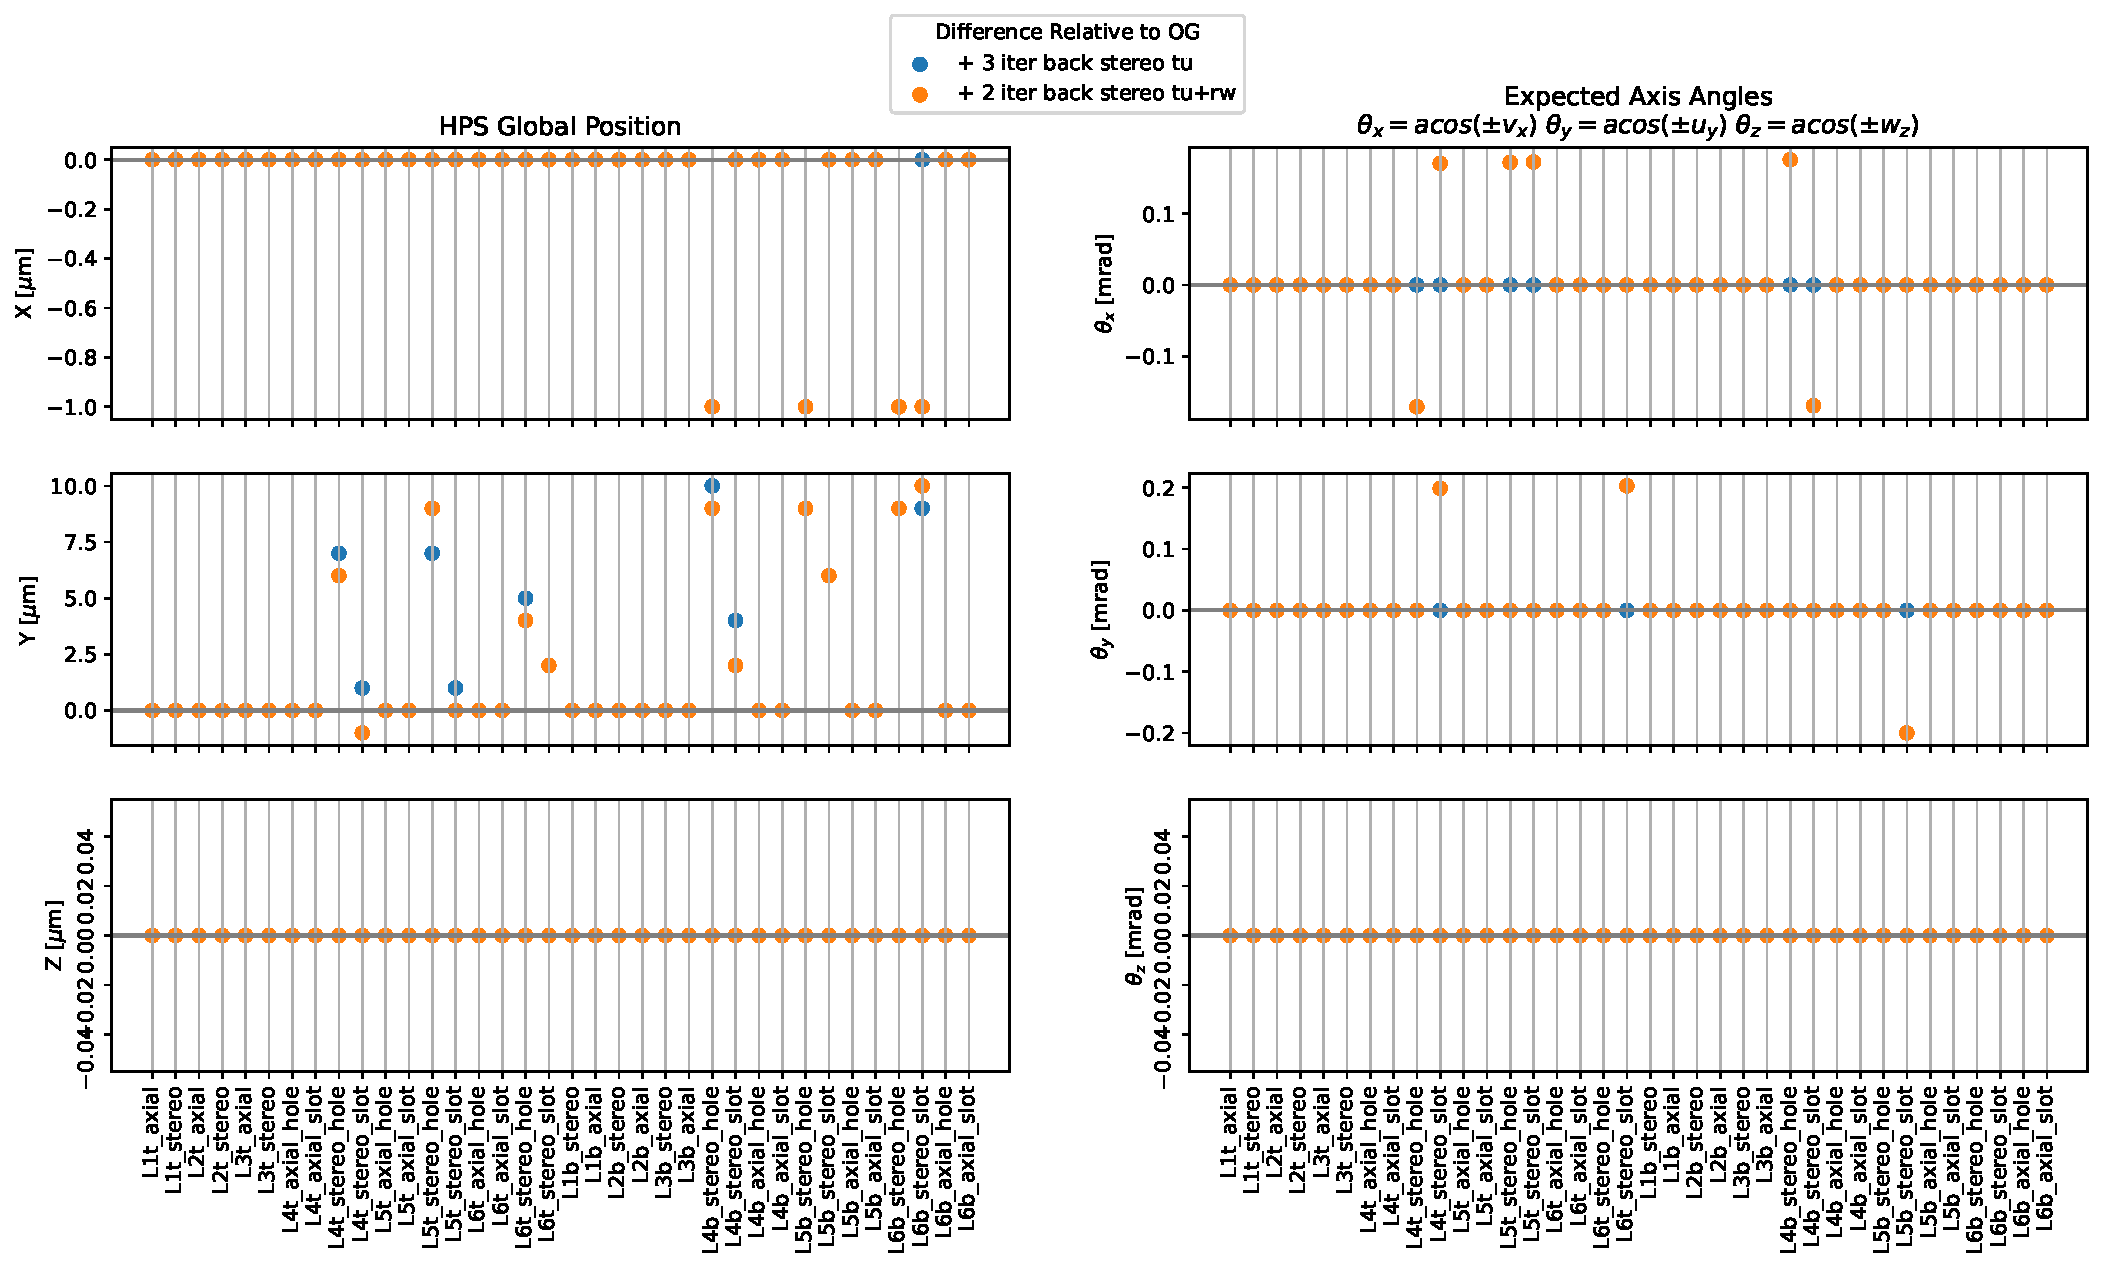
\includegraphics[width=\textwidth]{figures/hps/alignment/example-det-vis-diff.pdf}
  \caption{Plotting all six global coordinates completely specifying position and
    orientation of each of the sensors in the \ac{hps} tracking detector relative to
    the base detector ``OG'' from \cref{fig:example-det-vis-abs}. We can now observe
    the quantitative differences between the different versions.}
  \label{fig:example-det-vis-diff}
\end{figure}

\section{Results}
This movement of the sensor positions within our detector model is all well-and-good,
but we should actually be investigating how these movements affect the reconstructed
physical variables of tracks when using the updated detector model.
In general, the physical variables that should be investigated can depend on the
priorities of the experiment; for \ac{hps} we wish to inspect
\begin{itemize}
  \item Momentum Magnitude -- the total magnitude of the momentum of the reconstructed
    track is a key component in all analyses done with \ac{hps} data and thus is a
    priority to be well understood. Often, it is also common to inspect the momentum
    magnitude for different types of tracks so that it can be understood to in even
    finer detail. (i.e. $p$ vs $\tan\lambda$, $p$ vs $\phi$, $p$ separated by charge,
    etc.)
  \item Beamspot Position -- the extrapolation of the track back to the target is
    another helpful variable for analyses and can be checked directly since \ac{hps}
    has other means for estimating the beam spot on the target.
  \item Position at \ac{ecal} -- this is helpful for making sure the \ac{svt} and
    the \ac{ecal} are aligned relative to one another in the detector model.
\end{itemize}

Unfortunately, due to the number of possible parameters that could be tuned,
the possibility of improving the alignment of the tracking detector is something
that can always be done.
Thus, while there is often a current ``best'' detector model, future analyzers
may need to re-process data with a later (and hopefully improved) model that
would be expected to be more accurate to the real detector that data was taken with.
The results shown here are just this -- a snapshot of the progress in aligning the
\ac{hps} \ac{svt}.

\todo[find]{find some figures of unaligned vs aligned physical quantities to show
  that this process is necessary and helpful.}